\chapter{INTRODUCTION}
\label{chap:intro}

The installed capacity of solar power in the US continues to grow as a
result of aging coal and natural gas power plants, lower costs,
state renewable portfolio standards, and efforts to decarbonize the
electrical grid.
As shown in \Cref{fig:solarinstall}, this growth has been steady since 2010 and shows no signs of abating.

\begin{figure}[ht]
  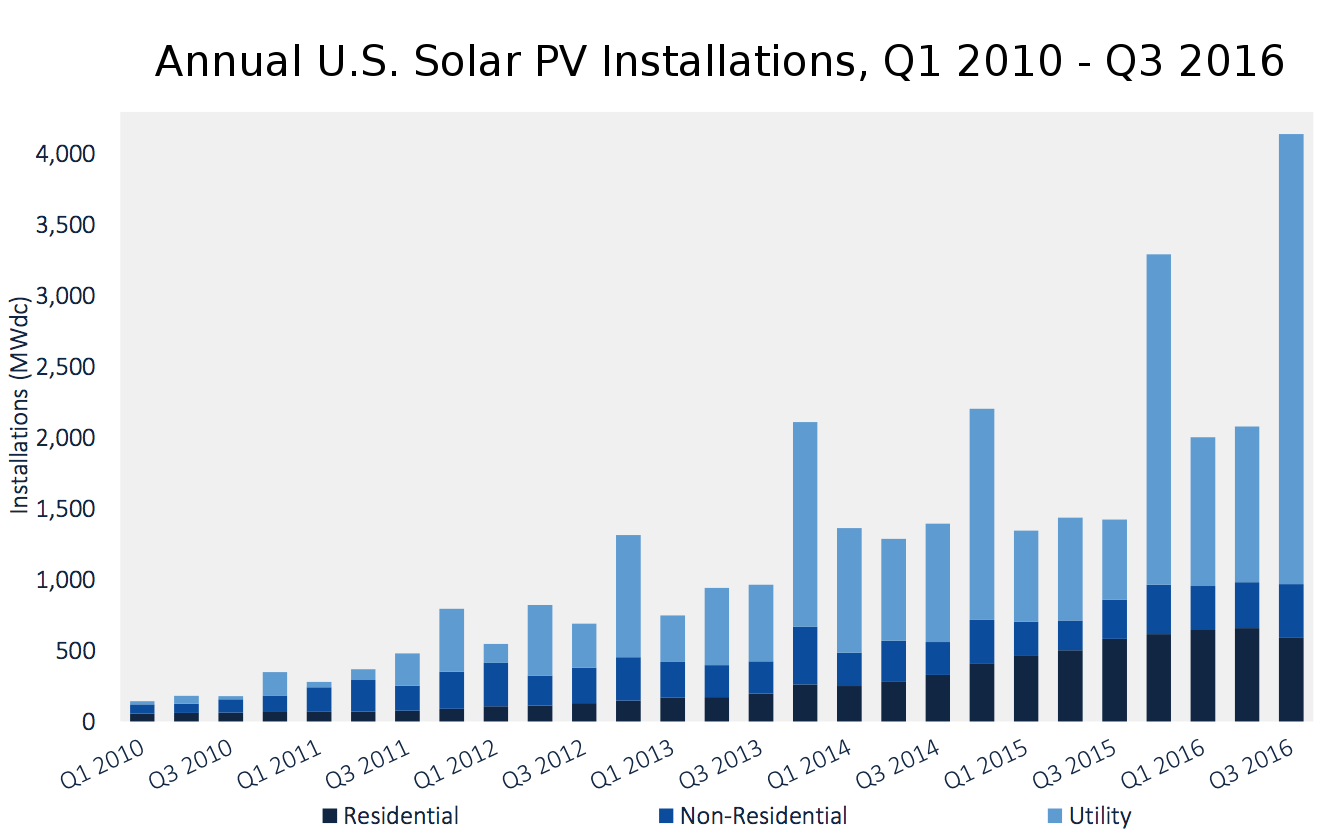
\includegraphics[width=\textwidth]{figs/solar_installations.png}
  \caption[Annual installations of solar PV in the US]{Annual
    installations of solar photovoltaic (PV) systems in the
    US. [Source:~\cite{GTM/SEIA2016}]}
\label{fig:solarinstall}
\end{figure}

Solar irradiance is the fuel that drives all solar power plants.
Unlike sources of fuel for conventional power generators like coal or
natural gas, the solar resource is highly variable due to the nature
of the chaotic system that is weather.
This variability of the solar resource leads to uncertainty at the
electric utility and increases management costs \citep{Joskow2011}.
Forecasts help utilities manage the variability in a number of ways
\citep{Kleissl2013,Inman2013}, including the optimal dispatch of
battery storage \citep{Cormode2015}.

This dissertation will explore solar irradiance forecasting at short
time horizons (now to two hours in the future) made possible by an
irradiance monitoring network.
First, the current state of solar power in the Southwest US and a
brief overview of forecasting methods will be discussed.

\section{State of Solar Power in the Southwest}
duck curve

a bit of SVERI analysis

how much solar total?
percentage of load?

nice heatmap

DG and visibility of DG


\section{Solar Irradiance Forecasting}
nowcasting DG

other techniques

little bit about WRF

\begin{figure}[h]
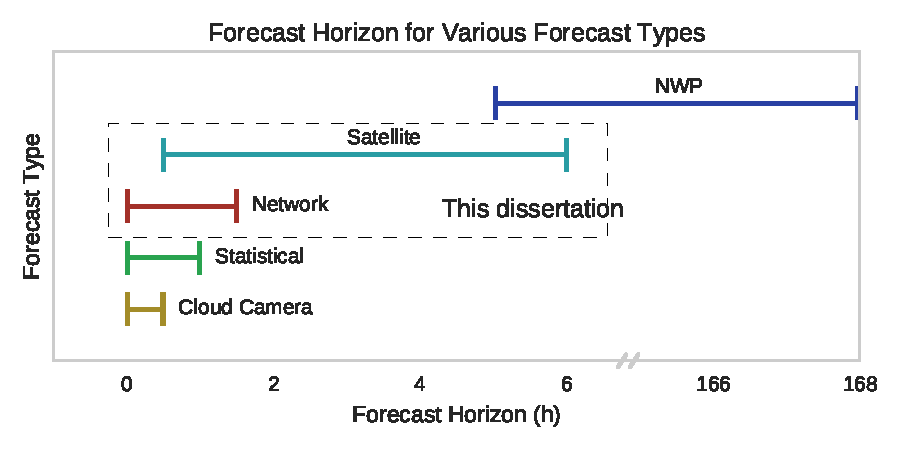
\includegraphics[width=\textwidth]{figs/fxhoriz.pdf}
\caption[Forecast horizon for various forecast types]{The optimal
  forecast horizons for various types of short-term forecasts. This
  dissertation will focus on network and satellite forecasts.}
\label{fig:fxhoriz}
\end{figure}


\section{This Dissertation in Brief}

\Cref{fig:bullshitplot} shows theoretical estimates of
forecast errors as a function of forecast horizon created near the
start of this dissertation work.
This dissertation works to analyze forecasting methods and measure
their relative errors as a function of forecast horizon in order to
produce the best forecasts for solar power in the Southwest.
\Cref{fig:newshitplot} shows the culmination of this work.
The dashed lines will beg studied in future work.

\begin{figure}[h]
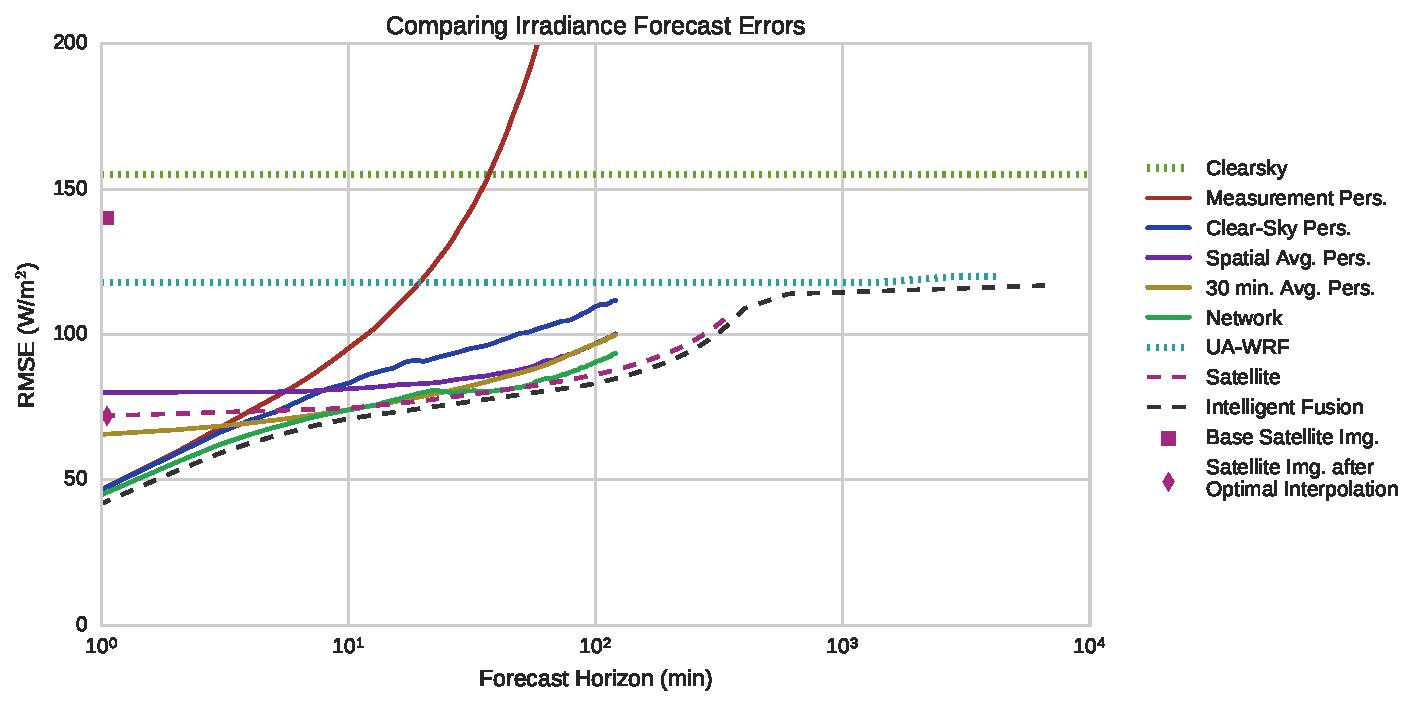
\includegraphics[width=\textwidth]{figs/timehorizon.pdf}
\caption[Irradiance forecast errors across forecast horizons]{A
  comparison of irradiance forecast root-mean squared errors (RMSE)
  across many time horizons. The solid lines (and points) indicate
  forecasts that will be studied in depth in this dissertation. Dashed
  lines are based on prelimnary analysis, but have not been studied in
  depth. Pers.\ refers to persistence, and UA-WRF refers to the
  numerical weather models generated at the UA using the Weather
  Research and Forecasting (WRF) model. The optimal grinding is a
  theoretical combination of forecasts at diffferent time horizons for
  the best forecast at all horizons. The persistence and network
  forecasts will be discussed in \Cref{chap:network} and the satellite
  image points will be discussed in \Cref{chap:satoi}.}
\label{fig:newshitplot}
\end{figure}

The specific forecasting methods studied in this dissertation rely on
a network of irradiance sensors.
A network with sufficient density and time resolution did not exist in
Tucson at the start of this dissertation work, so we set out to design
inexpensive sensors and to deploy them.
The design and deployment of the network is described in
\cref{chap:sens_net}.
For the period of April to July 2014, we collected data from about 50
custom sensors and rooftop PV systems to use in subsequent studies.

With this irradiance network data, the first forecasting methodology
we implemented and analyzed relies only on data from the network as
described in \cref{chap:network}.
This forecast is labeled as network in \cref{fig:newshitplot}.
On average this forecast shows a skill improvment of 20\% over a
reference persistence forecast.
The network forecast also nicely transitions from improving upon a
clear-sky persistence forecast at very short forecast horizons and an
area or time average persistence at longer horizons.

While analyzing this network forecast, we also carefully analyzed
various types of persistence forecasts to understand how the network
forecast works.
We found that smoother forecasts, or those with lower variance as
compared to the observations, may seem to perform better than
forecasts with higher variance when error metrics are considered in
isolation.
Using a Taylor diagram, we show that network forecasts transition from
matching the observation's variance to essentially becoming an area
average persistence forecast after about 20 minutes.

With short-term forecasts covered by the network forecasts, we began
studying forecasts derived from satellite images.
A number of algorithms exist that convert images of the tops of clouds
from geostationary satellites to images of irradiance on the ground.
Naturally, this conversion from cloud top brightness to the amount of
radiation that passes through clouds is error prone.
We found that these satellite derived irradiance estimates from a
current image (pink square on left axis of \cref{fit:newshitplot}),
before any forecasting is involved, had errors nearly as large as
always assuming a clear sky.
It is unlikely that producing a forecast from such a nowcast would
reduce errors, so satellite derived forecasts would quickly become
worse than a clear-sky forecast, at least in terms of RMSE.
Thus, in order to produce high quality forcasts from satellite derived
irradiance images, we first improved the satellite derived irradiance
nowcasts.

Better satellite derived irradiance nowcasts were generated by again
using data from the irradiance sensor network as described in
\cref{chap:satoi}.
Using a data assimilation method known as optimal interpolation, we
combined the sensor data with the satellite derived irradiance based
on the relative errors between them.
We also parameterized the correlations between pixels in the satellite
images in various ways.
These correlations are responsible for spreading information from the
sensor locations to other locations throughout the image.

We found significant improvements using this method after various
complicating factors such as misalignment in the satellite image
relative to the ground sensors were corrected.
The improved nowcasts RMSE is shown as the pink diamond in
\cref{fig:newshitplot} and is almost half of the RMSE for the
uncorrected images.
We also found that this method to improve satellite irradiance
nowcasts is applicable to a number of satellite to irradiance
algorithms.

To produce forecasts of irradiance in future work, one might use a
forecasting method that relies on only cloud advection.
With a forecasting model in place, optimal interpolation can be
extended to the Kalman filter with constantly incorporates new data
into a forecast while also retaining information about past data.
It is common in numerical weather prediction to use an ensemble of
states to propogate and Kalman filter.
An ensemble in this case also allows for each forecast to have a
different cloud motion field which may improve the final forecasts.

Satellite forecasts have been shown to perform well for forecast
horizons up to 6 hours.
For longer forecast horizons, numerical weather models are likely
needed.
We currently run the Weather Research and Forecasting (WRF) model with
a custom configuration for Arizona.
Improvements in the WRF model may come from assimilating satellite
data, data from the sensor network, or studying WRF ensembles.

Finally, once high-quality forecasts are available for all forecast
horizons, they can be intellgently fused to produce a single forecast
that incorporates the best properties of each forecast methodology.
Utilities and other stakeholders often need these fused forecasts to
make decisions.





%%% Local Variables:ah
%%% mode: latex
%%% TeX-master: "dissertation"
%%% End:
